\chapter{Technical Specification}
\section{Protocol}

In this section, we provide an explanation of the protocol and the values used in it.

The protocol of our signing service consists of five main phases:

\begin{itemize}
	\item Pre-Login (see~\ref{subsec:pre-login})
	\item Login (see~\ref{subsec:login})
	\item Post-Login (see~\ref{subsec:post-login})
	\item Signature Generation (see~\ref{subsec:signature-generation})
	\item Signature Verification (see~\ref{subsec:signature-verification})
\end{itemize}

For a high-level overview of these phases, see figure~\ref{fig:highlevelprotocoloverview}.

\begin{figure}
	\begin{center}
		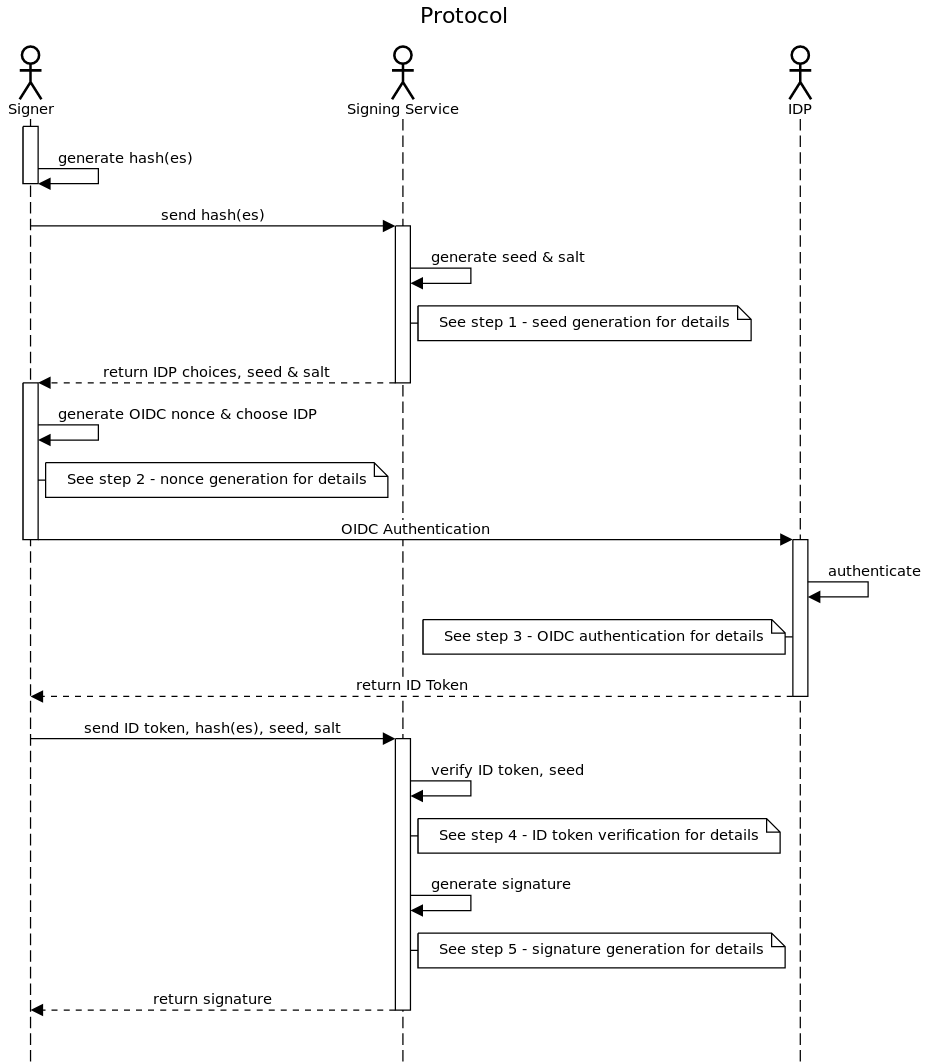
\includegraphics[scale=0.5]{images/protocol_signature_generation_high_level.png}
		\caption{High-level protocol overview}
		\label{fig:highlevelprotocoloverview}
	\end{center}
\end{figure}

\subsection{Pre-Login}\label{subsec:pre-login}
In this phase the signer provides a list of hashes to signing service
(this list may consist of just one entry in case the signer wishes to sign a single document).

Then, the signing service generates a random \texttt{seed}.

\[ seed = random() \]

This \texttt{seed}, together with a static \texttt{secret} known to the server only,
is used to calculate the key that is used to generate a \gls{HMAC}
of the sorted list\footnote{The list has to be sorted,
otherwise the same hash values in a different order would produce different \gls{HMAC}s.} of hashes.
The key is calculated using a \gls{HKDF} as specified in RFC~5869~\cite{rfc5869}.

\[ hmacKey = HKDF(seed, staticServerSecret) \]

From the key obtained from the \gls{HKDF} and the document hashes,
a salt value is derived by using a \gls{HMAC} as specified in RFC~2104~\cite{rfc2104}.

\[ salt = HMAC(hmacKey, sorted(hashes)) \]

Next, the nonce is calculated by masking each hash with the salt by using a \gls{HMAC},
and hashing this list with a secure hash algorithm.


\[ nonce = H(\{\ HMAC(salt, h) \ \ \forall \ h \in sorted(hashes)\ \}) \]

The nonce needs to be derived from the list of salted hashes because
only the salted hashes will be included in the signature file.


\paragraph{Purpose of the salt}
The salt is used to mask the document hashes in the \gls{OIDC} nonce from the \gls{IDP}.
This way the \gls{IDP} cannot learn whether two people sign the same document(s).
If we wouldn't salt the hashes, the \gls{OIDC} nonce would be the same for the same sorted list of hashes,
and the \gls{IDP} could detect when two people sign the same document(s).

While someone could argue that the IDP server learning about different people signing the same document
isn't much of a security problem, we want to ensure that each involved party is given the absolute minimum
of information necessary for them to fulfil their role\footnote{as specified in the non-functional requirements, "Protection of Information"}.

In addition to shielding the hashes from the \gls{IDP},
the salt masks the document hashes from recipients of multi-file signatures.
When multiple files are signed at once, all of the hashes are included in the resulting signature file.
However, since someone could receive only a subset of the files that were signed together,
they could learn the document hashes of the other files.
(For example, a company signing a thousand invoices at once but sending each customer only their invoice.)

Again, this shouldn't be a significant problem but again, we don't want to allow this.
So we include only the salted hashes in the signature file, and the salt itself.

Since the verifier is in possession of the document(s), they can calculate their respective hashes,
and then derive the salted hash(es) themselves since the salt is included in the signature file.
Then they can check whether their document hash(es) are in the list of salted hashes.
This way, they can verify their document(s) without learning anything about the other documents,
not even their hash values.

\paragraph{Purpose of the seed}
The seed is necessary in order to obtain a different \gls{HMAC} key for every request
despite using the same static secret on the server,
and in order to strengthen the \gls{HKDF} as recommended in RFC~5869~\cite[Section 3.1]{rfc5869}.
Furthermore, the seed is used as a \gls{CSRF} protection mechanism without the need for the server to keep any state.
If no such \texttt{seed} were used for generating the salt,
the signing server would be forced to keep the \gls{CSRF} token in memory and link it to the users session,
in order to be able to check whether the hashes or the salt were replaced somewhere in the \gls{OIDC} authentication implicit flow
(and as such, establishing the secure link between the document hashes and the authentication).
If the signing server didn't verify this,
it would allow for skipping the Pre-Login step (see~\ref{subsec:pre-login})
and proceeding directly to the Post-Login step (\ref{subsec:post-login}) as seen from the signing service.

The server then returns a list of \gls{IDP} choices as well as the \texttt{seed} and the \texttt{salt} to the client.

For a sequence diagram of this phase, see figure~\ref{fig:seedgenerationstep}.

\begin{figure}
	\begin{center}
		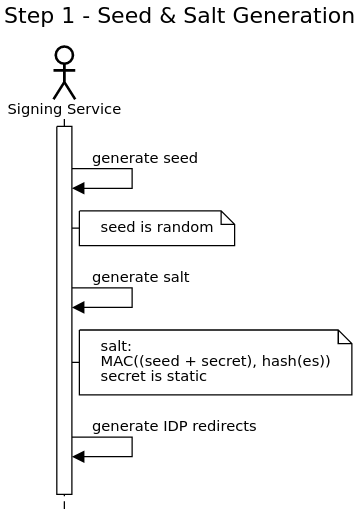
\includegraphics[scale=0.5]{images/protocol_step1_seed_generation.png}
		\caption{Seed generation step}
		\label{fig:seedgenerationstep}
	\end{center}
\end{figure}

\subsection{Login}\label{subsec:login}
TODO update graphic: no client-side generating anything because no one likes to write javascript
For a graphical representation of this, see figure~\ref{fig:noncegenerationstep}.

Having received a list of \gls{IDP}s from the server, the client chooses an \gls{IDP} and follows the link.
The user then authenticates with the \gls{IDP} and receives their ID token as seen in figure~\ref{fig:oidcauthenticationstep}.

\begin{figure}
	\begin{center}
		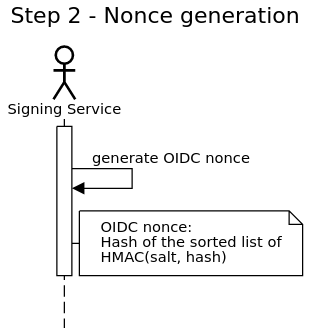
\includegraphics[scale=0.5]{images/protocol_step2_nonce_generation.png}
		\caption{Nonce generation step}
		\label{fig:noncegenerationstep}
	\end{center}
\end{figure}

\begin{figure}
	\begin{center}
		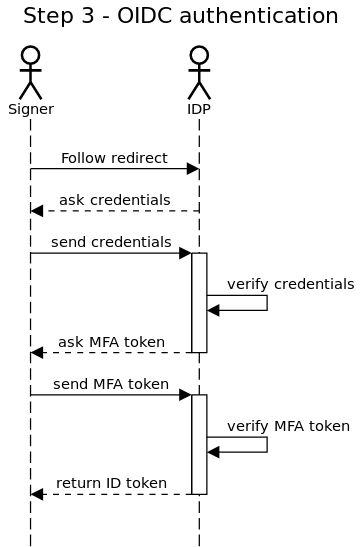
\includegraphics[scale=0.5]{images/protocol_step3_oidc_authentication.png}
		\caption{OIDC authentication step}
		\label{fig:oidcauthenticationstep}
	\end{center}
\end{figure}

\subsection{Post-Login}\label{subsec:post-login}
As shown in figure~\ref{fig:tokenverificationstep},
the client sends the ID token, the list of hashes, the \texttt{seed} and the \texttt{salt} to the signing service.
The signing service then verifies the \texttt{salt}, OIDC nonce and ID token as described in~\ref{subsubsec:verificationhashesseedsalt}.
After this step, the \texttt{seed} is not used anymore and should be discarded.


\subsubsection{Verification of hashes, seed and salt}\label{subsubsec:verificationhashesseedsalt}
Upon receiving a well-formed request in the format described in~\ref{subsubsec:signrequest},
the signing server performs no fewer than the following checks:
\begin{enumerate}
	\item Verifying the id\_token as described in~\cite[Section~7.2]{rfc7519}
	\item Checking the length of the seed and salt values
	\item Checking that the salt and nonce match the calculation described in~\ref{subsec:pre-login}
\end{enumerate}
These verifications are paramount to the safety of the system.

\begin{figure}
	\begin{center}
		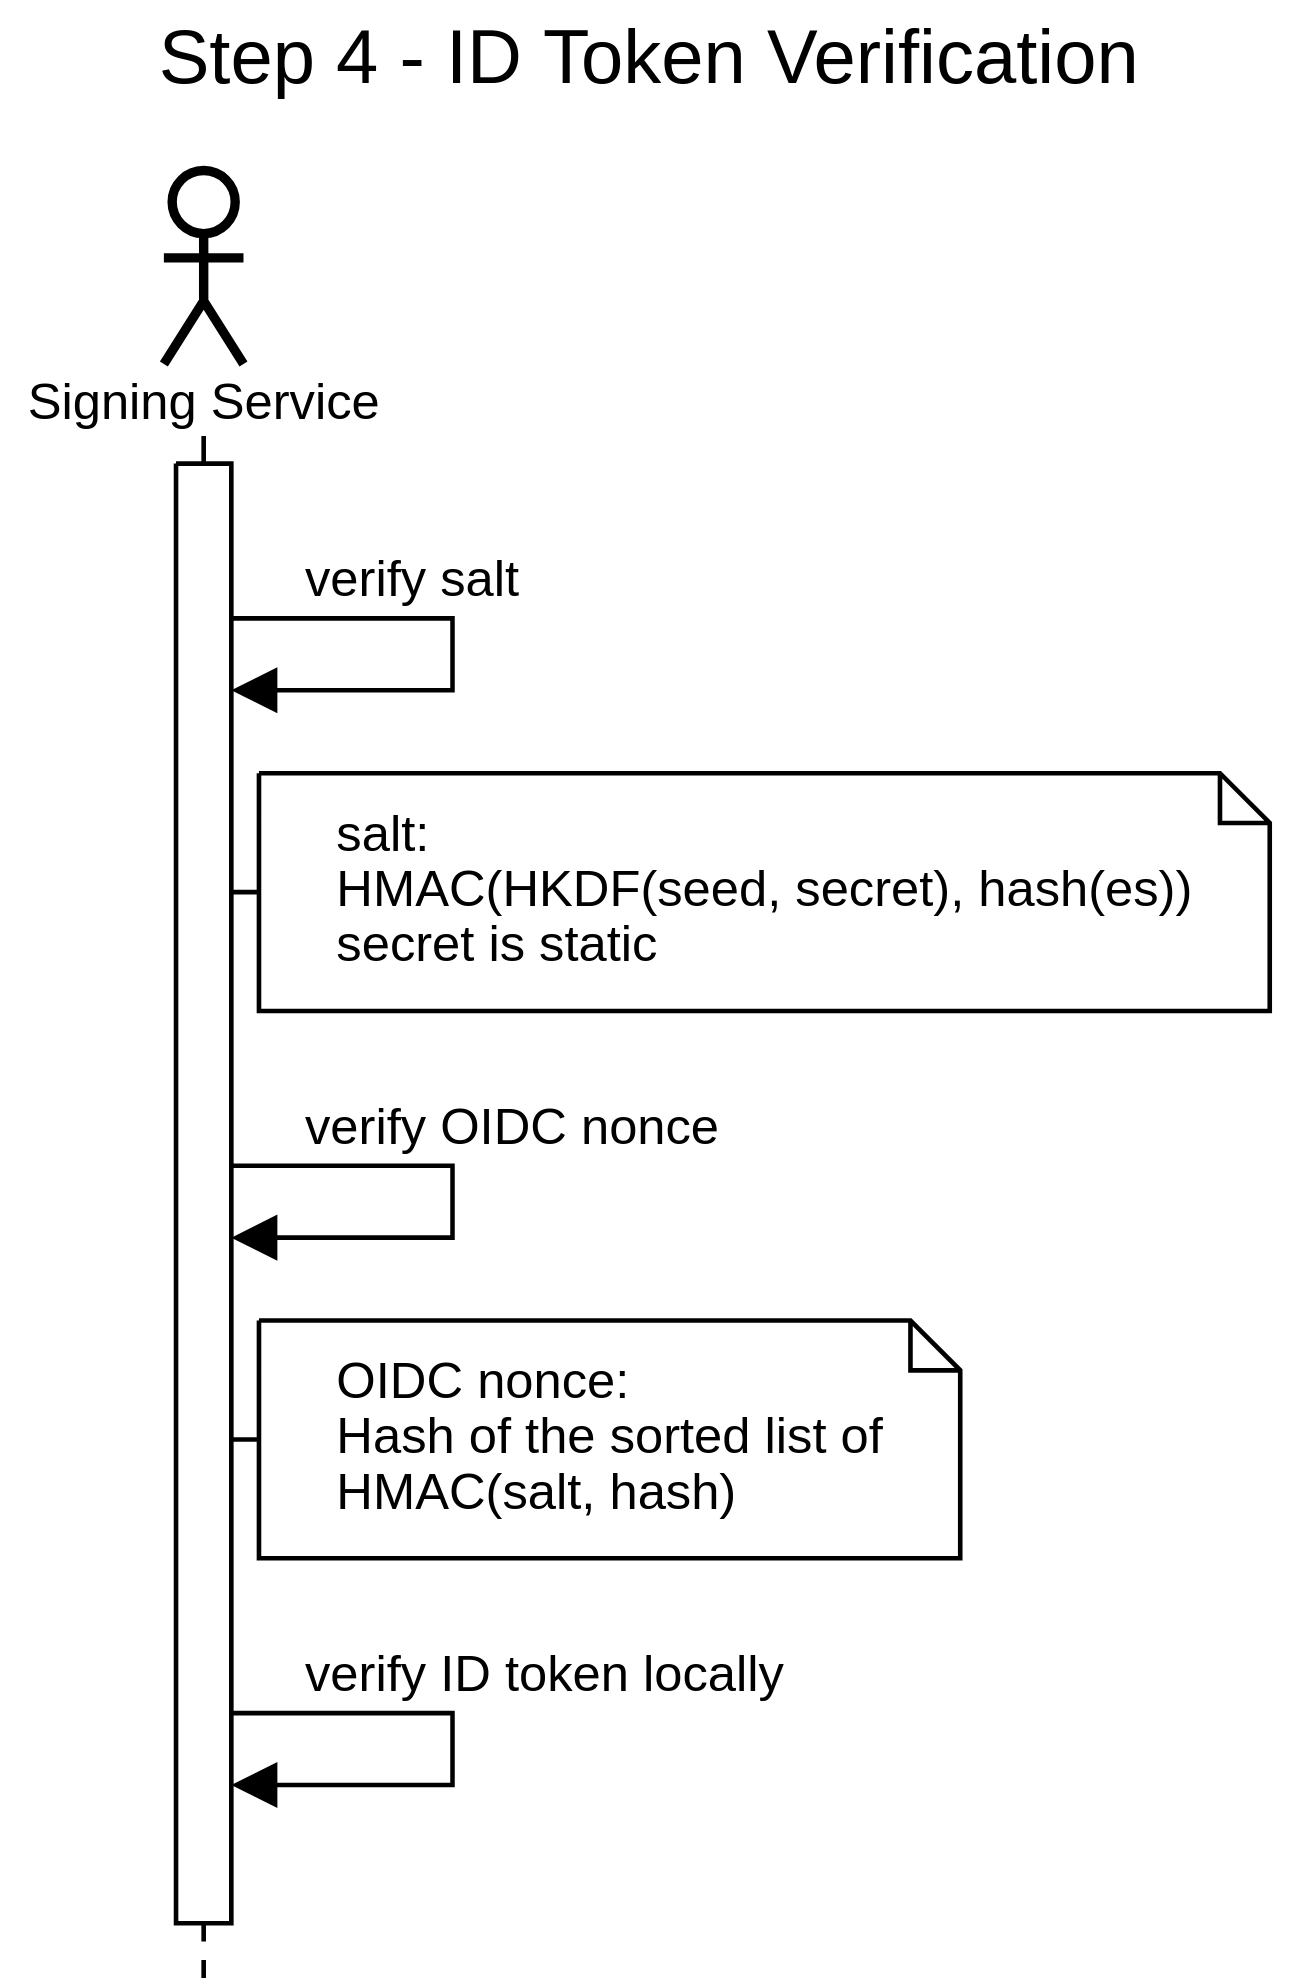
\includegraphics[scale=0.5]{images/protocol_step4_id_token_verification.png}
		\caption{Token verification step}
		\label{fig:tokenverificationstep}
	\end{center}
\end{figure}

\subsection{Signature Generation}\label{subsec:signature-generation}
The signing server requests a new signing key from the \gls{HSM}, which in turn generates a private key and returns a \gls{CSR}.
This \gls{CSR} is sent to the \gls{CA} where it is signed and the signed certificate returned.

Each hash is then submitted to the \gls{HSM} to be signed by the signing key.

Then, for each hash an intermediate signature file consisting of the signed hash,
the ID token, the \texttt{salt} and a sorted list of all other salted hashes is created.
The hash of this file is sent to a \gls{TSA} where a signed timestamp is created and returned.

Finally, the signed timestamp, and all the certificate chains,
\gls{OCSP} responses and \gls{CRL}s of the involved parties,
is added to signature file, which is then returned to the user.

TODO update this figure since we no longer loop
See figure~\ref{fig:signaturegenerationstep} for a sequence diagram of this process.

\begin{figure}
	\begin{center}
		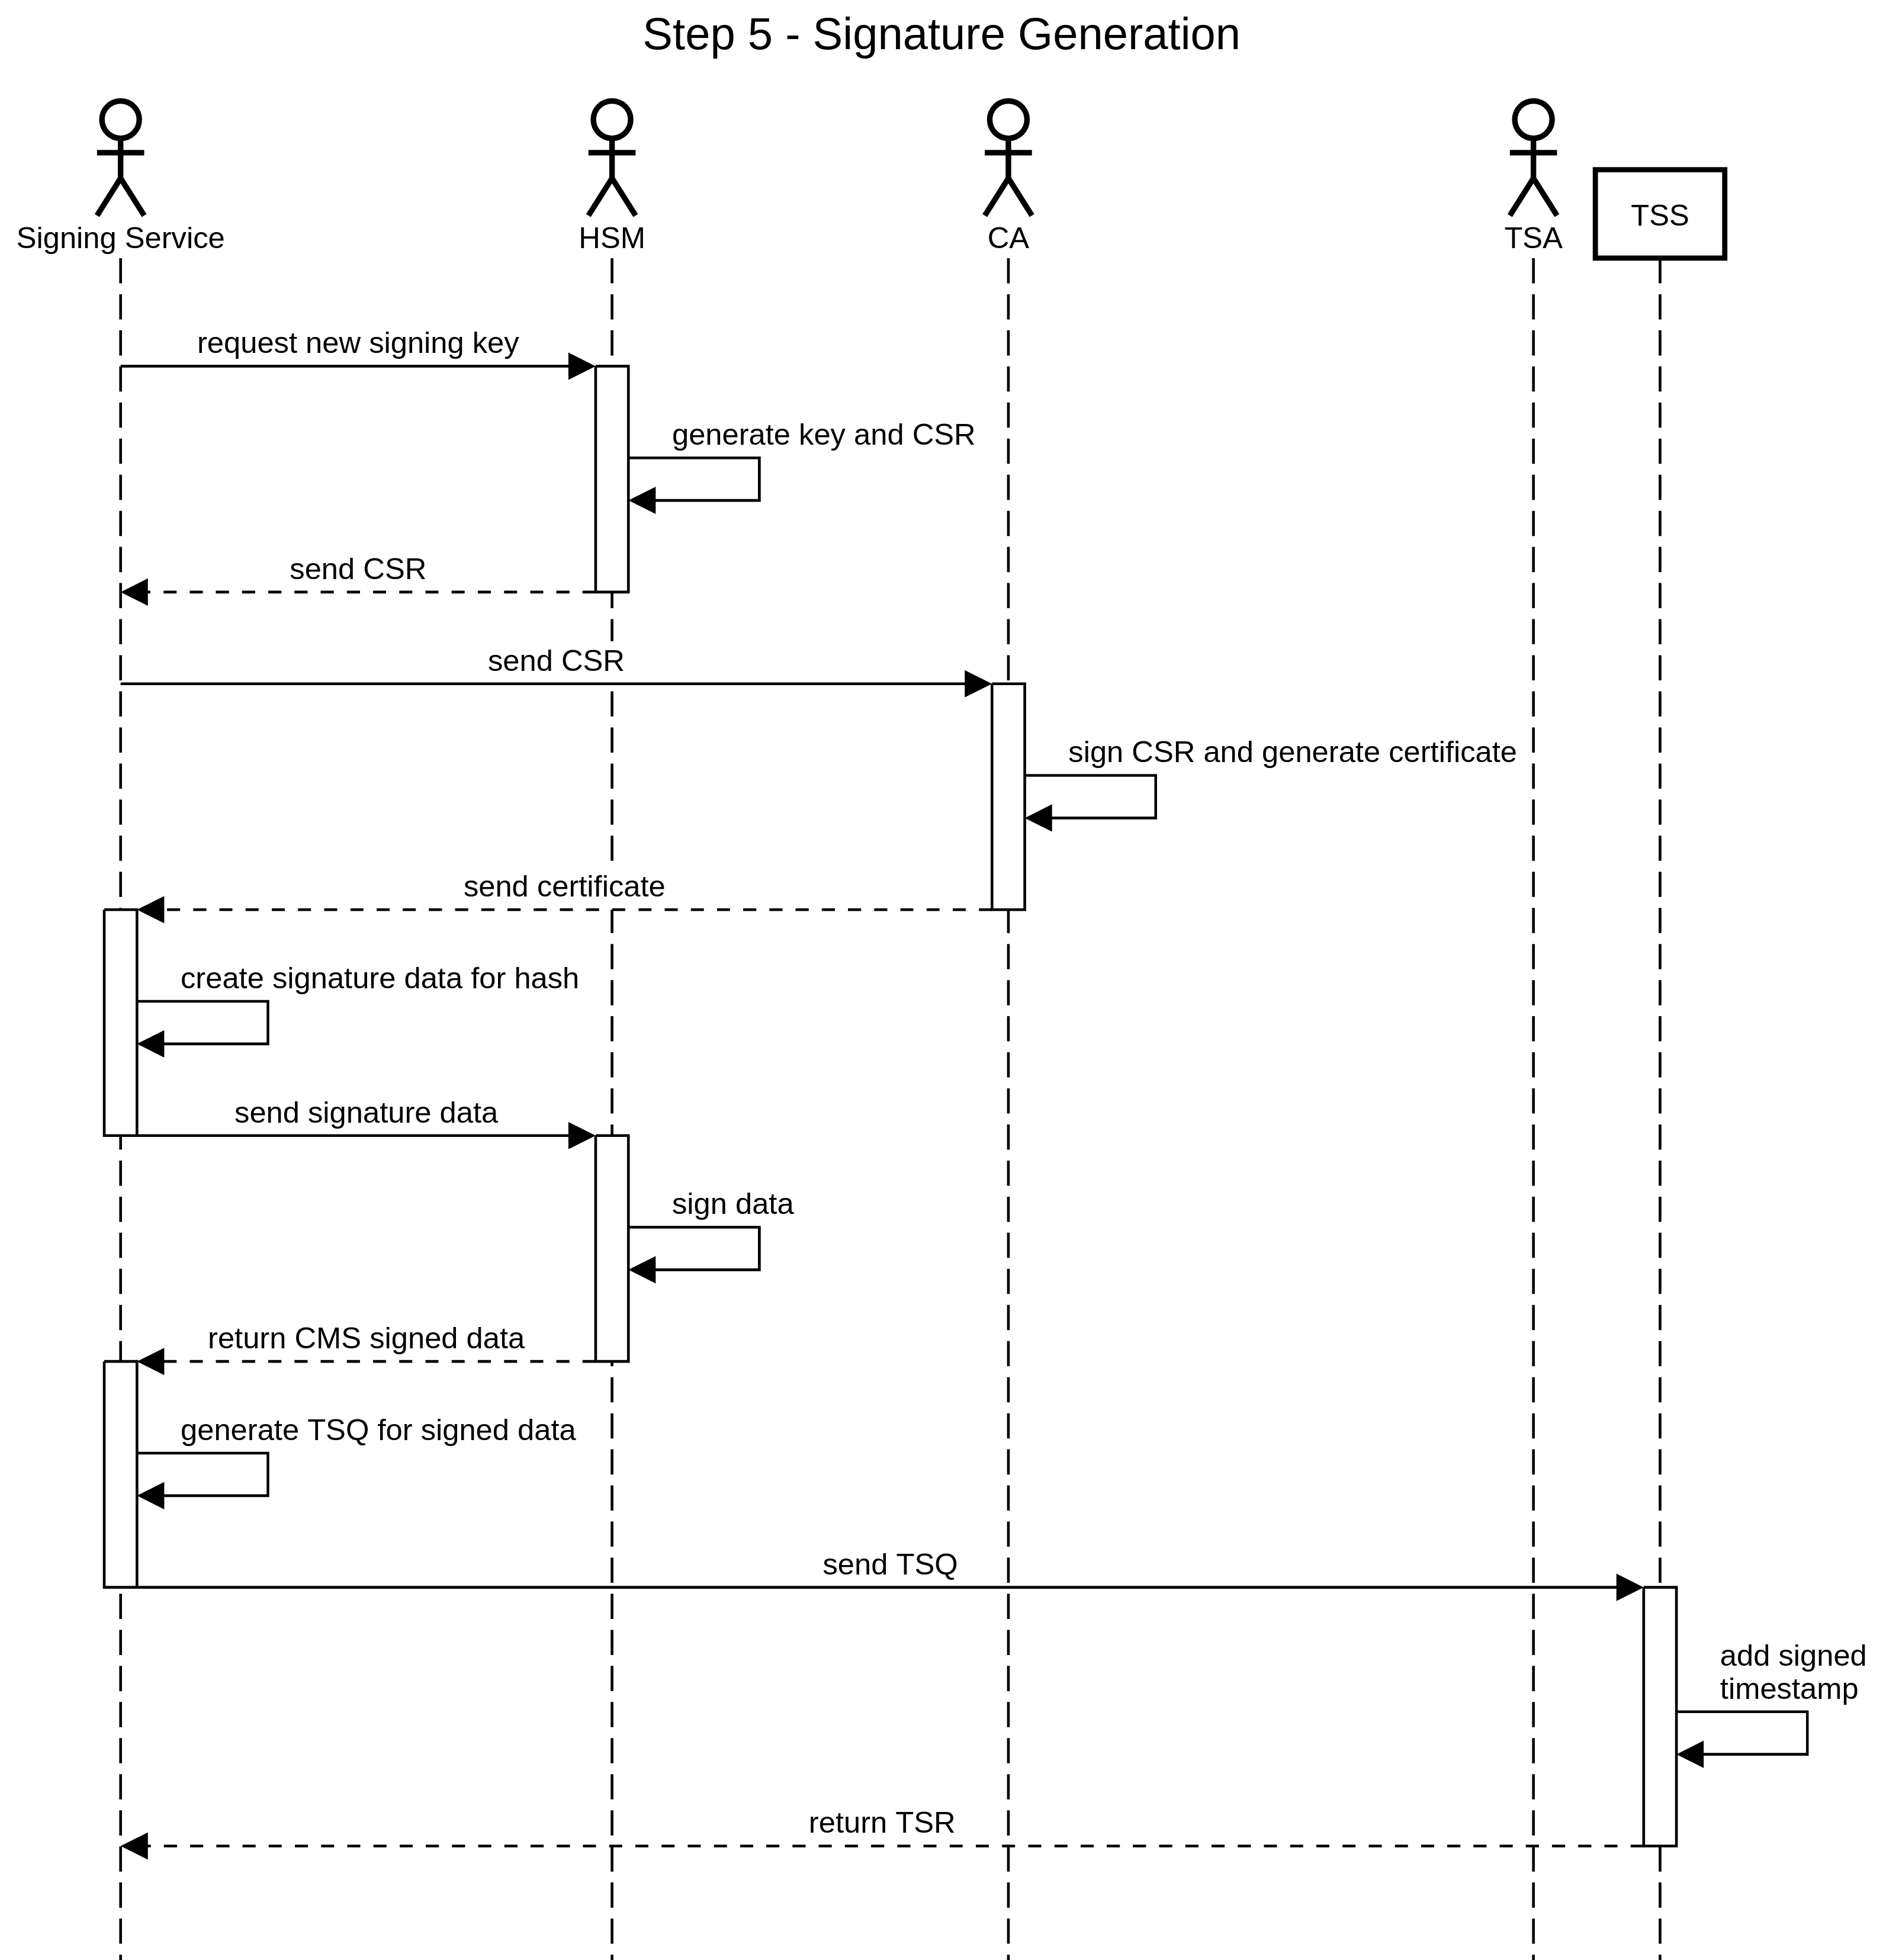
\includegraphics[scale=0.45]{images/protocol_step5_signature_generation.png}
		\caption{Signature generation step}
		\label{fig:signaturegenerationstep}
	\end{center}
\end{figure}

\subsection{Signature Verification}\label{subsec:signature-verification}

The signature verification can either be online (figure~\ref{fig:onlinesignatureverificationprotocol})
or offline (figure~\ref{fig:offlinesignatureverificationprotocol}).

For online verification, the user simply uploads the list of hashes and the signature file to the verification service.

\begin{figure}
	\begin{center}
		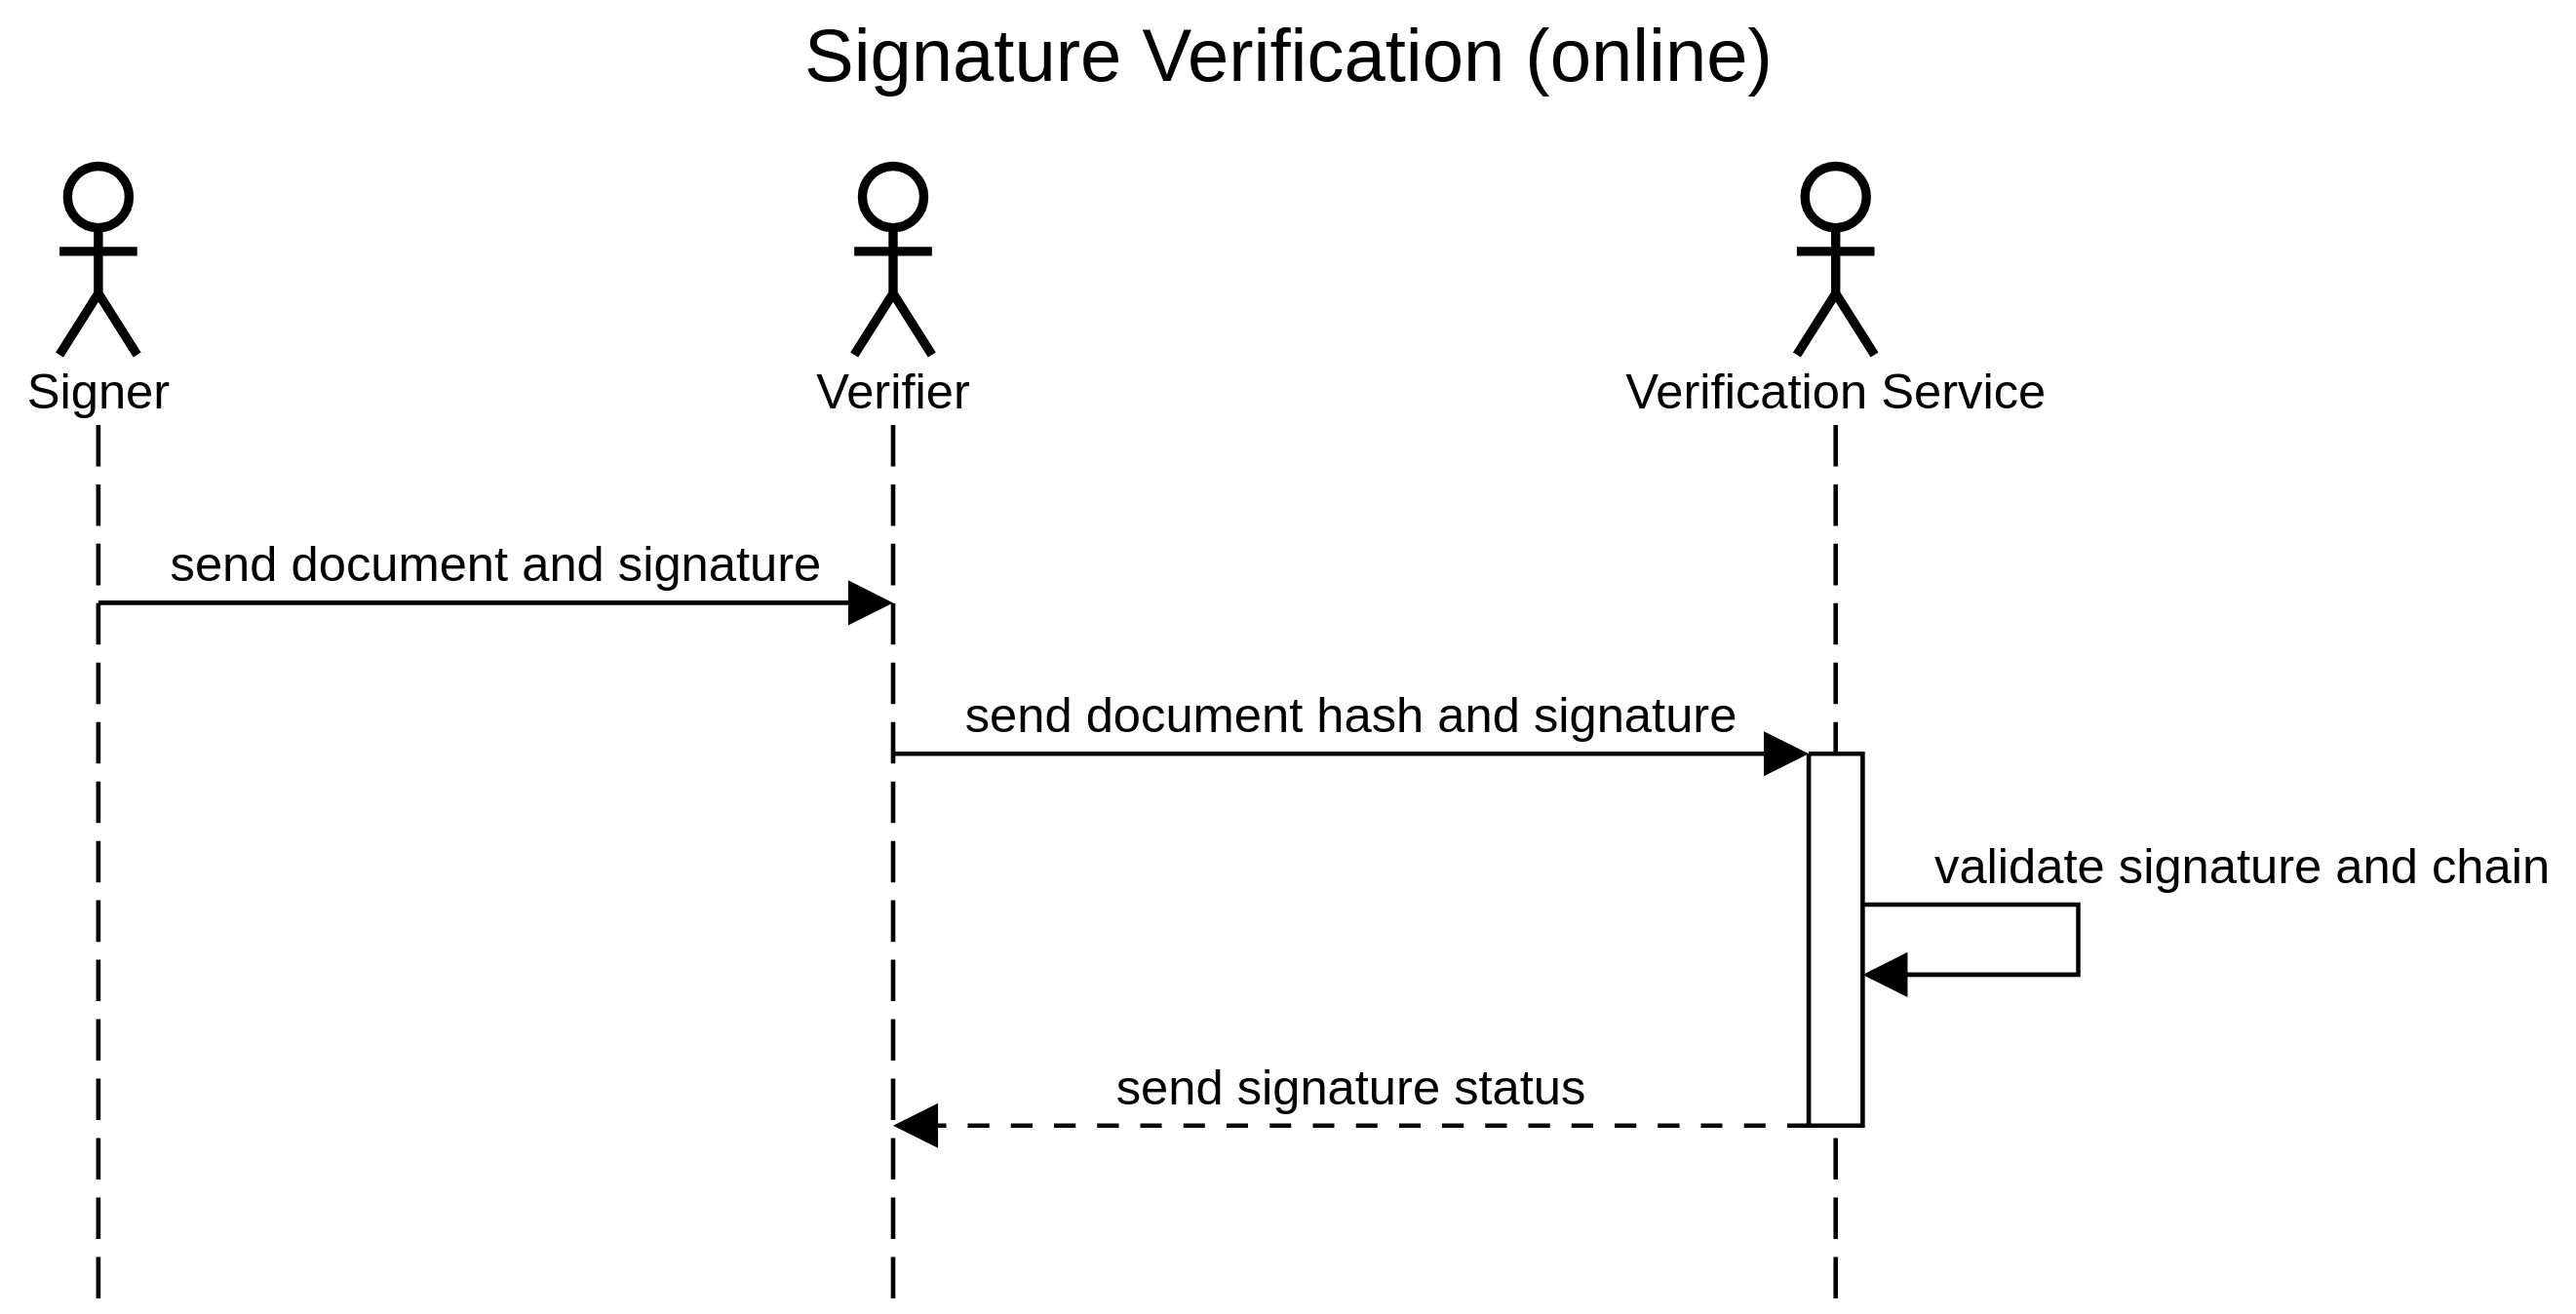
\includegraphics[scale=0.5]{images/protocol_online_verification_high_level.png}
		\caption{Online Signature Verification Protocol}
		\label{fig:onlinesignatureverificationprotocol}
	\end{center}
\end{figure}

For the offline verification, the user downloads the verification programme and starts it.
Then, they upload the list of hashes and signature file just as if they were using online verification,
but to their own copy of the verification service running on their computer without needing any network connection
instead of a remote verification service.

\begin{figure}
	\begin{center}
		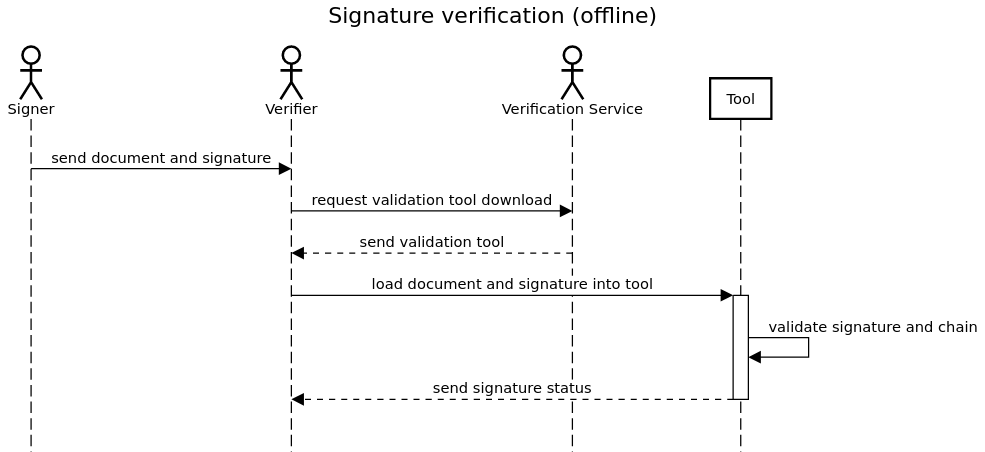
\includegraphics[scale=0.5]{images/protocol_offline_verification_high_level.png}
		\caption{Offline Signature Verification Protocol}
		\label{fig:offlinesignatureverificationprotocol}
	\end{center}
\end{figure}

To verify a signature,
the verifier first needs to verify the chain of signed timestamps and their respective \gls{CA} chains (figure~\ref{fig:timestampverificationstep}).

\begin{figure}
	\begin{center}
		% TODO update this figure since we no longer loop
		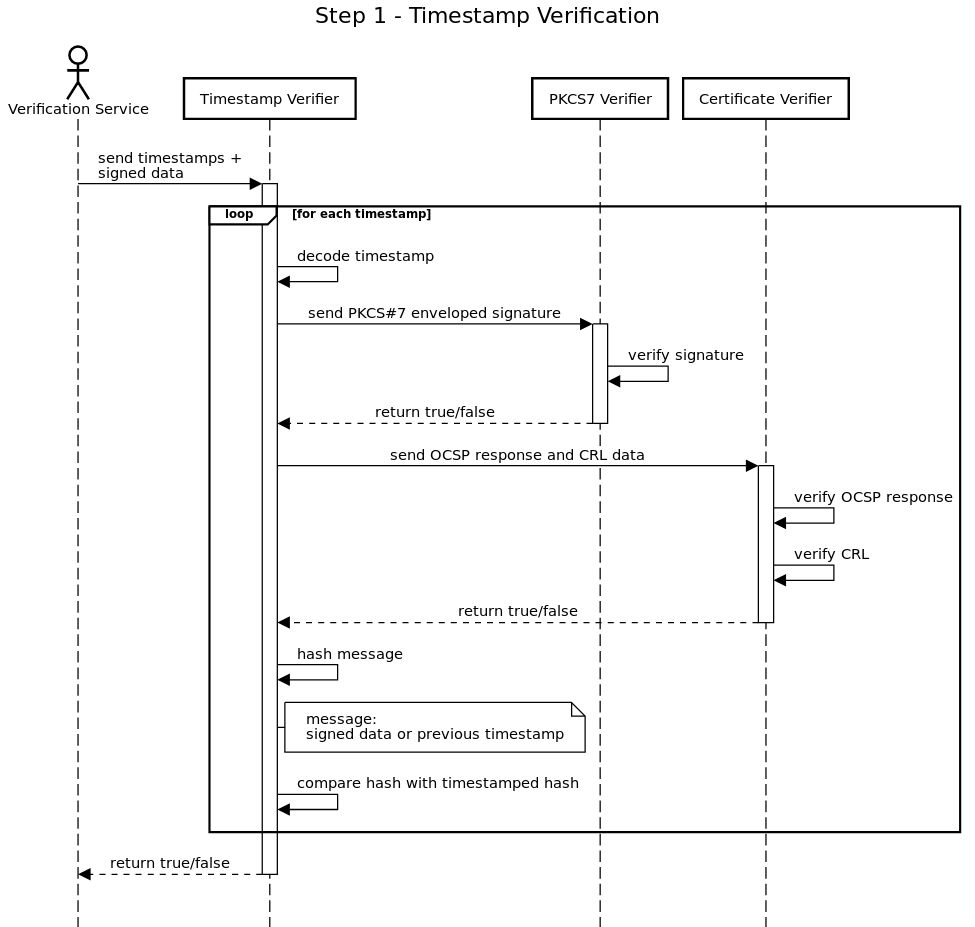
\includegraphics[scale=0.5]{images/protocol_verification_step1_timestamp.png}
		\caption{Timestamp verification step}
		\label{fig:timestampverificationstep}
	\end{center}
\end{figure}

The signature itself can then be verified (figure~\ref{fig:signaturegenerationstep}), along with
the certificate chain for the signing certificate.

\begin{figure}
	\begin{center}
		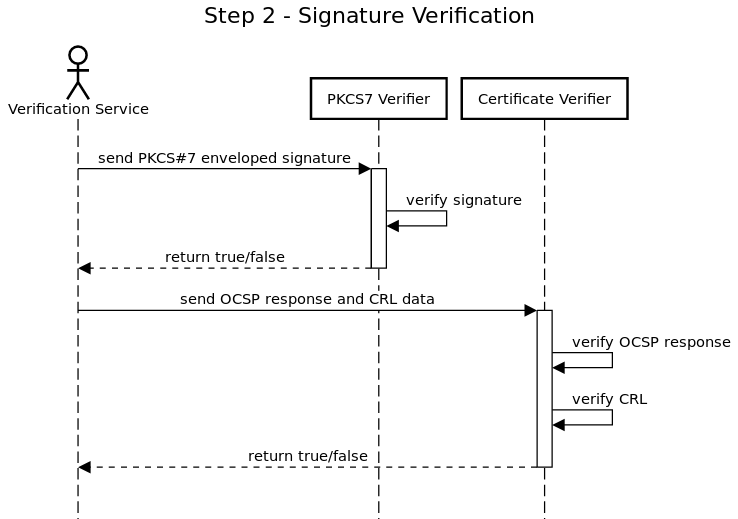
\includegraphics[scale=0.5]{images/protocol_verification_step2_signature.png}
		\caption{Signature verification step}
		\label{fig:signatureverificationstep}
	\end{center}
\end{figure}

Then, the ID token itself needs to be verified,
as well as the certificate chain of the key used to sign the ID token (figure~\ref{fig:idtokenverification}).

\begin{figure}
	\begin{center}
		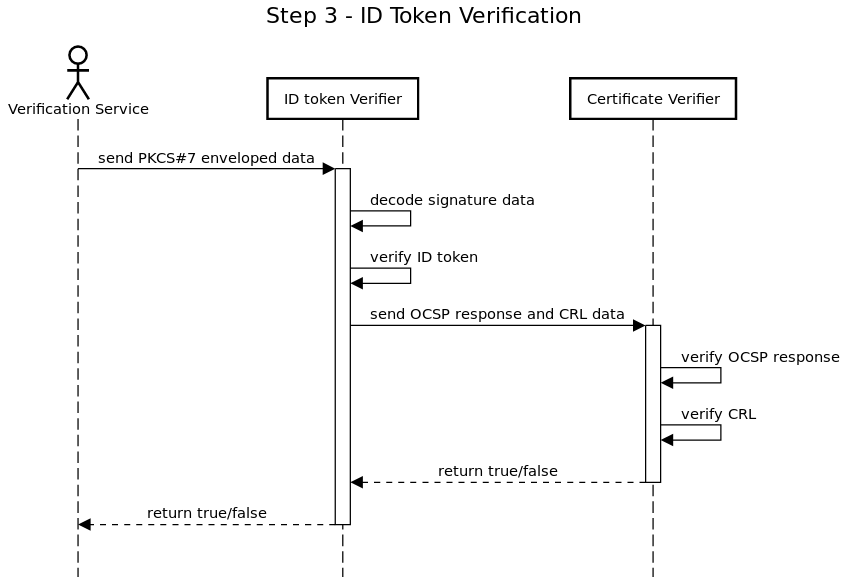
\includegraphics[scale=0.5]{images/protocol_verification_step3_id_token.png}
		\caption{ID token verification}
		\label{fig:idtokenverification}
	\end{center}
\end{figure}

In order to verify the link of the document hashes with the ID token,
the document hash needs to be salted, inserted into the sorted list of the other salted hashes,
and the resulting list hashed again.
The result must be the same as the nonce in the ID token.
At last, the hash of the document must match the included hash.
Figure~\ref{fig:signaturedataverification} illustrates this process.

\begin{figure}
	\begin{center}
		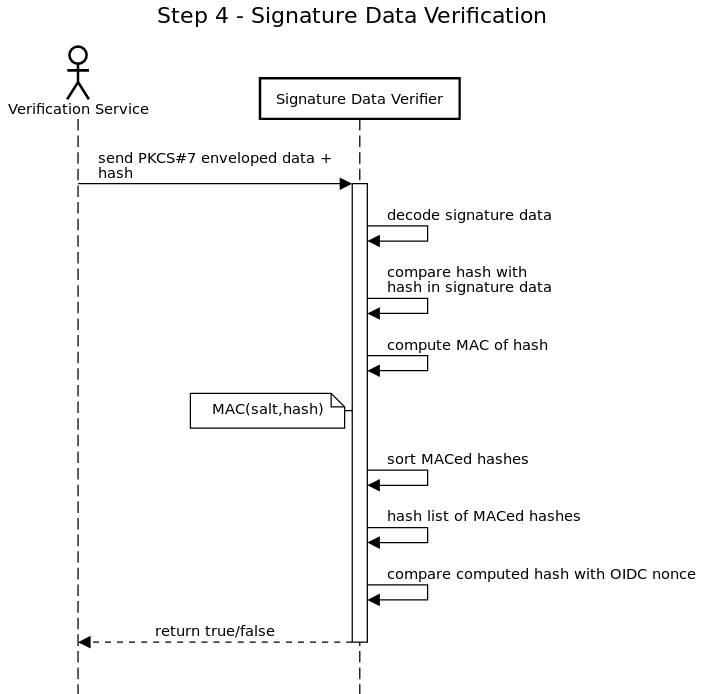
\includegraphics[scale=0.5]{images/protocol_verification_step4_signature_data.png}
		\caption{Signature data verification}
		\label{fig:signaturedataverification}
	\end{center}
\end{figure}

\section{REST API}\label{sec:rest-api}
In this section the \gls{REST} \gls{API} is specified:
Which endpoints are offered, what they expect as input data and what they respond with.
The examples are given for illustration purposes and are not normative.

\subsection{Signing Service}
The signing service offers the following endpoints:

\begin{longtable}{|l|l|l|l|}
	\hline
	\textbf{No.} & \textbf{Endpoint} & \textbf{Method} & \textbf{Description} \\ \hline
	1 & /api/v1/login & POST & Send hashes to sign, receive list of OIDC providers \\ \hline
	2 & /api/v1/sign & POST & Send hashes to sign, receive signature URL \\ \hline
	3 & /api/v1/signatures/:id & GET & Retrieve signature file \\ \hline
\caption{Endpoints offered by the Signing Service}
\end{longtable}

In the most common case, the client application will call these endpoints in the order listed:
\begin{enumerate}
	\item The user submits the hashes of the documents they wish to sign and receives a list of IDPs
	\item After authentication with the IDP, the user submits the hashes again, this time the server will begin construction of the signature file
	\item After the signature is created, the user downloads the file to their device
\end{enumerate}

But, the order in which these endpoints are used is not enforced by the API except for what is required with the \gls{OIDC} implicit flow,
and the linkage of the id\_token with the signing.

\subsubsection{Client errors}
\label{apiclienterrors}
If a malformed request is sent by the client, the signing server will respond with a 400 client error code,
and a message indicating the cause of failure.
This format of returning errors is the same for all endpoints of the signing server.

\begin{longtable}{|l|l|l|l|}
	\hline
	\textbf{Parameter} & \textbf{Presence} & \textbf{Type} & \textbf{Description} \\ \hline
    message & MANDATORY & String & Reason for rejection of request \\ \hline
	\caption{Output in case of invalid input}
\end{longtable}

Sample Error Response:
\begin{lstlisting}[caption={Error response}, captionpos=b, language=JavaScript, label={lst:hashesresponse}]
	HTTP/1.1 400 Bad Request
	Content-Type: application/json

	{
             "message": "Invalid hash length"
	}
\end{lstlisting}

\subsubsection{login}
This endpoint is used for submitting the hashes the user wishes to sign.

\begin{longtable}{|l|l|l|l|}
	\hline
	\textbf{Parameter} & \textbf{Presence} & \textbf{Type} & \textbf{Description} \\ \hline
	hashes & MANDATORY & List<String> & Hashes of the documents to be signed \\ \hline
    \caption{Input to the login endpoint}
\end{longtable}

Duplicates in the list of hashes are not allowed and are rejected by the API as described in~\ref{apiclienterrors}.
The length of each hash is checked, and if they don't match the hashing algorithm used the request is rejected as well.
The encoding of the hashes is checked, and if they don't appear to be a string of sane hex numbers the request is rejected.

Output:

\begin{longtable}{|l|l|l|l|}
	\hline
	\textbf{Parameter} & \textbf{Presence} & \textbf{Type} & \textbf{Description} \\ \hline
	providers & MANDATORY & Map<String, Url> & List of providers with the redirect url \\ \hline
	seed & MANDATORY & String & Seed for generating the salt \\ \hline
	salt & MANDATORY & String & Salt for generating the OIDC nonce \\ \hline
	\caption{Output of the login endpoint}
\end{longtable}

Sample Request:
\begin{lstlisting}[caption={login request}, captionpos=b, language=JavaScript, label={lst:hashesrequest}]
POST /api/v1/hashes HTTP/1.1
Host: service.example.org
Content-Type: application/json

{
  "hashes": [
	  "e8a96e6203b9c0df058ba862abc63d9c520157faef6d5d54e54e526b0a85b2be",
	  "0b9a7fd3e612061a7fe6d834e102a143170f33d0e8c5a8eb79416aa3eb53c0d6"
  ]
}
\end{lstlisting}

Sample Response:
\begin{lstlisting}[caption={login response}, captionpos=b, language=JavaScript, label={lst:hashesresponse}]
HTTP/1.1 201 Created
Content-Type: application/json

{
  "providers": {
  	"SwissID": "https://...&nonce=6cd7ef99e5e79d68d681e5d097b7f805381c4d013152fa3f26d06bd728ae49fa",
	"Google": "https://...&nonce=6cd7ef99e5e79d68d681e5d097b7f805381c4d013152fa3f26d06bd728ae49fa"
  },
  "seed": "84c97acc49335faa0266fb29b4228205e9400a85a10faa68ec30cf894e1730ed",
  "salt": "cfb663431af5e2d68be48867f93e86e477cd7eeefc10b16a51c238d2c810561b"
}
\end{lstlisting}

\subsubsection{sign}\label{subsubsec:signrequest}
After having authenticated with the IDP, the client application calls the signing endpoint.
This is where the actual signature file is being assembled by the signing server.

\begin{longtable}{|l|l|l|l|}
	\hline
	\textbf{Parameter} & \textbf{Presence} & \textbf{Type} & \textbf{Description} \\ \hline
	id\_token & MANDATORY & string & OIDC ID token \\ \hline
	seed & MANDATORY & String & Seed for generating the salt \\ \hline
	salt & MANDATORY & String & Salt for generating the OIDC nonce \\ \hline
	hashes & MANDATORY & List<String> & Hashes of the documents to be signed \\ \hline
	\caption{Input to the signing endpoint}
\end{longtable}

The signing server performs no fewer than the following checks, and if any of them fail to pass,
the server rejects the request as described in as described in~\ref{apiclienterrors}.
\begin{itemize}
    \item The input \gls{JSON} is checked against the expected format
	\item The \gls{JWT} id\_token is verified as described in~\cite[Section~7.2]{rfc7519}
	\item The seed, salt, hashes, and the nonce in the id\_token are verified as described in~\ref{}
\end{itemize}

Output:

\begin{longtable}{|l|l|l|l|}
	\hline
	\textbf{Parameter} & \textbf{Presence} & \textbf{Type} & \textbf{Description} \\ \hline
	signature url & MANDATORY & Url & Url to the generated signature file\\ \hline
	\caption{Output of the signing endpoint}
\end{longtable}

Sample Request:
\begin{lstlisting}[caption={sign request}, captionpos=b, language=JavaScript, label={lst:signrequest}]
POST /api/v1/sign HTTP/1.1
Host: service.example.org
Content-Type: application/json

{
  "idtoken": {...},
  "seed": "84c97acc49335faa0266fb29b4228205e9400a85a10faa68ec30cf894e1730ed",
  "salt": "cfb663431af5e2d68be48867f93e86e477cd7eeefc10b16a51c238d2c810561b",
  "hashes": [
    "e8a96e6203b9c0df058ba862abc63d9c520157faef6d5d54e54e526b0a85b2be",
    "0b9a7fd3e612061a7fe6d834e102a143170f33d0e8c5a8eb79416aa3eb53c0d6"
  ]
}
\end{lstlisting}

Sample Response:

\begin{lstlisting}[caption={sign response}, captionpos=b, language=JavaScript, label={lst:signresponse}]
HTTP/1.1 201 Created
Content-Type: application/json

{
	"signature": "https://signingservice.local/api/v1/signatures/0b1131c417cafcc5a5f259d357903026f8e0c4f85e3ca0b68f3d55b8e32a55e8"
}
\end{lstlisting}

\subsubsection{signatures/:id}
Input:

\begin{longtable}{|l|l|l|l|}
	\hline
	\textbf{Parameter} & \textbf{Presence} & \textbf{Type} & \textbf{Description} \\ \hline
	id & MANDATORY & String & id of the hash that was signed \\ \hline
    \caption{Input to the signature retrieval endpoint}
\end{longtable}

Output:

\begin{longtable}{|l|l|l|l|}
	\hline
	\textbf{Parameter} & \textbf{Presence} & \textbf{Type} & \textbf{Description} \\ \hline
	signature & MANDATORY & String & Base64 encoded signature for the requested hash \\ \hline
	\caption{Output of the signature retrieval endpoint}
\end{longtable}

Sample Request:

\begin{lstlisting}[caption={signature request}, captionpos=b, language=JavaScript, label={lst:signaturerequest}]
GET /api/v1/signatures/e8a96e62034e526b0a85b2be HTTP/1.1
Host: service.example.org
\end{lstlisting}

Sample Response:

\begin{lstlisting}[caption={signature response}, captionpos=b, language=JavaScript, label={lst:signatureresponse}]
HTTP/1.1 200 OK
Content-Type: application/json

{
  "signature": "IyMjIFJFU1QgQVBJIFNwZWNpZmljYXRpb24gU2NyYXRjaHBhZAoKIyMjIyBQcmUtQXV0aCBlbmRw...b2ludCAKIyMjIyMgRW5kcG9pbnQKYGBgUE9TVCAvYXBpL3YxL3NpZ25gYGAK"
}
\end{lstlisting}

\subsection{Verification Service}
Endpoints:

\begin{longtable}{|l|l|l|}
	\hline
	\textbf{Endpoint} & \textbf{Method} & \textbf{Description} \\ \hline
	/api/v1/verify & POST & Send hash signature file for verification \\ \hline
	\caption{Overview of endpoints offered by the verification service}
\end{longtable}

\subsubsection{verify}
Input:

\begin{longtable}{|l|l|l|l|}
	\hline
	\textbf{Parameter} & \textbf{Presence} & \textbf{Type} & \textbf{Description} \\ \hline
	hash & MANDATORY & String & Hash of the signed document \\ \hline
	signature & MANDATORY & String & base64 encoded signature file \\ \hline
    \caption{Input to the signature verification endpoint}
\end{longtable}

Output:

\begin{longtable}{|l|l|l|l|}
	\hline
	\textbf{Parameter} & \textbf{Presence} & \textbf{Type} & \textbf{Description} \\ \hline
	valid & MANDATORY & Boolean & validity of signature \\ \hline
	error & OPTIONAL & String & error message why the signature is invalid \\ \hline
	\caption{Output of the signature verification endpoint}
\end{longtable}

Sample Request:
\begin{lstlisting}[caption={sign request}, captionpos=b, language=JavaScript, label={lst:verifyrequest}]
POST /api/v1/sign HTTP/1.1
Host: service.example.org
Content-Type: application/json

{
  "hash": "e8a96e6203b9c0df058ba862abc63d9c520157faef6d5d54e54e526b0a85b2be",
  "signature": "IyMjIFJFU1QgQVBJIFNwZWNpZmljYXRpb24gU2NyYXRjaHBhZAoKIyMjIyBQcmUtQXV0aCBlbmRw...b2ludCAKIyMjIyMgRW5kcG9pbnQKYGBgUE9TVCAvYXBpL3YxL3NpZ25gYGAK"
}
\end{lstlisting}

Sample Response:

\begin{lstlisting}[caption={sign response}, captionpos=b, language=JavaScript, label={lst:verifyresponse}]
HTTP/1.1 200 OK
Content-Type: application/json

{
  "valid": true
}
\end{lstlisting}

Invalid signature:

\begin{lstlisting}[caption={sign response}, captionpos=b, language=JavaScript, label={lst:verifyresponsefailed}]
HTTP/1.1 200 OK
Content-Type: application/json

{
  "valid": false,
  "error": "signed hash and provided hash don't match"
}
\end{lstlisting}

\section{Signature File Format}
TODO
\subsection{Long-Term Validation}
\gls{LTV} allows for the validation of signatures long after the document was signed~\cite{etsipades}.

We need \gls{LTV} for two main reasons:
\begin{enumerate}
    \item Imagine if the \gls{CA} were revoked that was used for the signatures: all signatures created using the same \gls{CA} would become invalid instantly, making countless documents, constracts and the like unverifiable.
    \item Extending the validity of the signature beyond the lifetime of the \gls{CA} used to sign it, for signatures that need to remain valid and verifiable for a very long time.
\end{enumerate}
In order for us to achieve this, all required elements for signature validation must be embedded into the signature file.
Without the addition of these elements, a signature can only be validated for a limited time.
This limitation occurs because the \gls{CA}s eventually expire, or get revoked.
Once the \gls{CA} certificate has expired, the issuing authority is no longer responsible for providing the revocation status information on that certificate.
Without the confirmed revocation status information on the signing keys, the signature cannot be validated.

To overcome this limitation, the following information has to be embedded into the signature:
\begin{enumerate}
    \item A timestamp on the signature
    \item The signing certificate
    \item The certificates used and their revocation status (\gls{OCSP} and \gls{CRL})
    \item An archive timestamp of the previous content
\end{enumerate}

The archive timestamp establishes the date in which the information collected was issued.
Provided the archive timestamp is valid,
we can be sure that the revocation information was issued at that time,
and check the validity of the signing certificate and the \gls{CA} certificate chain.
Thus we can be certain that it was not revoked at the point in time the document was signed.
This allows us to extend the validity of the signature past the expiration time of the \gls{CA}.

However, this does not extend the validity of the signature indefinitely,
it merely extends the expiration until the expiration time of the timestamping authority's certificate.

For many cases this may be enough, but it doesn't quite allow for long-time archival yet.
When the timestamping certificates' expiration is impending,
the signature expiration time has to be extended by adding another timestamp signed by a \gls{CA} not yet close to expiration.
This re-stamping has to be repeated periodically in order to keep the signature valid and verifiable.
This allows for near-indefinite archival.

